\documentclass{article}
\usepackage{fancyhdr}
\usepackage{extramarks}
\usepackage{amsmath}
\usepackage{amssymb}
\usepackage{enumerate}
\usepackage{graphicx}
\usepackage{pgfplotstable}
\usepackage{listings}
\usepackage{braket}
\lstset{framexleftmargin=5mm, frame=shadowbox, rulesepcolor=\color{blue}}


\topmargin=-0.45in
\evensidemargin=0in
\oddsidemargin=0in
\textwidth=6.5in
\textheight=9.0in
\headsep=0.25in

\linespread{1.1}

\pagestyle{fancy}
\lhead{\hmwkAuthorName}
\chead{\hmwkClass\ : \hmwkTitle}
\rhead{\firstxmark}
\lfoot{\lastxmark}
\cfoot{\thepage}

\renewcommand\headrulewidth{0.4pt}
\renewcommand\footrulewidth{0.4pt}

\setlength\parindent{24pt}

%
% Create Problem Sections
%

\newcommand{\enterProblemHeader}[1]{
    \nobreak\extramarks{}{Problem \arabic{#1} continued on next page\ldots}\nobreak{}
    \nobreak\extramarks{Problem \arabic{#1} (continued)}{Problem \arabic{#1} continued on next page\ldots}\nobreak{}
}

\newcommand{\exitProblemHeader}[1]{
    \nobreak\extramarks{Problem \arabic{#1} (continued)}{Problem \arabic{#1} continued on next page\ldots}\nobreak{}
    \stepcounter{#1}
    \nobreak\extramarks{Problem \arabic{#1}}{}\nobreak{}
}

\setcounter{secnumdepth}{0}
\newcounter{partCounter}
\newcounter{homeworkProblemCounter}
\setcounter{homeworkProblemCounter}{1}
\nobreak\extramarks{Problem \arabic{homeworkProblemCounter}}{}\nobreak{}

%
% Homework Problem Environment
%
% This environment takes an optional argument. When given, it will adjust the
% problem counter. This is useful for when the problems given for your
% assignment aren't sequential. See the last 3 problems of this template for an
% example.
%
\newenvironment{homeworkProblem}[1][-1]{
    \ifnum#1>0
        \setcounter{homeworkProblemCounter}{#1}
    \fi
    \section{Problem \arabic{homeworkProblemCounter}}
    \setcounter{partCounter}{1}
    \enterProblemHeader{homeworkProblemCounter}
}{
    \exitProblemHeader{homeworkProblemCounter}
}

%
% Homework Details
%   - Title
%   - Due date
%   - Class
%   - Section/Time
%   - Instructor
%   - Author
%

\newcommand{\hmwkTitle}{Homework\ \#10}
\newcommand{\hmwkDueDate}{April 27, 2015}
\newcommand{\hmwkClass}{PHYS 5243 - Solid State Physics}
\newcommand{\hmwkClassInstructor}{Professor Sheena Murphy}
\newcommand{\hmwkAuthorName}{Chase Brown}


\begin{document}

\begin{homeworkProblem}
	\section{Atomic Hole doping of Graphene on SiC - Tight Binding Calculation Compared with ARPES data}
		 A study on single layered graphene on SiC has shown that epitaxial graphene is doped by the substrate through charge transfer.\cite{gierz2008atomic}  In the case of SiC, the Fermi level is shifted up such that the graphene is n-doped  by approximately 420 meV.  Angle resolved photoemmission spectra (APRES) shows direct observation of the band structure of the graphene.  Here we show that the band structure for graphene is not greatly altered from the tight binding theory predictions, while the Fermi level shifts dramatically back to the zero point by the addition of Bismuth.
		 
		\subsection{Single Layer Tight Binding Calculations}
			To begin, we start with the Brillouin Zone of Graphene, shown below.

			\begin{center}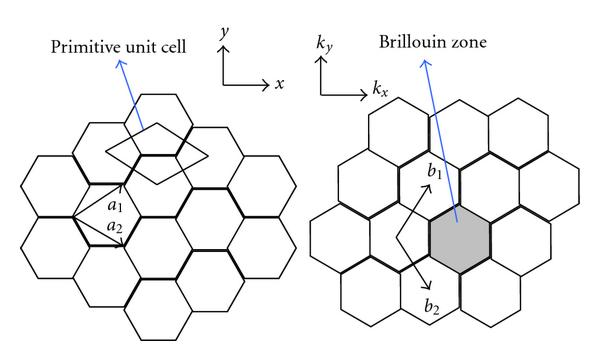
\includegraphics[scale=2]{BZ_Graphene.jpg}\end{center}
			
			The distance between carbon atoms in real space is $a = 0.142$ nm, therefore we can see that the primitive lattice vectors are:
			
			\begin{center} $\textbf{a}_1 = \frac{a}{2} (3,\sqrt{3})$ and $\textbf{a}_2 = \frac{a}{2} (3,-\sqrt{3})$ \end{center}
			
			Taking the Fourier Transform of real space, we find that the lattice vectors for the reicprocal space are:
			
			\begin{center} $\textbf{b}_1 = \frac{2\pi}{3a} (1,\sqrt{3})$ and $\textbf{b}_2 = \frac{2\pi}{3a} (1,-\sqrt{3})$ \end{center}
			
			Starting with the assumption of a linear combination of atomic orbitals (LCAO), we find the ground state of an single electron $\psi_\textbf{k}(\textbf{r})$ moving through a potential of an isolated atom $U(\textbf{r})$.  We then notice that if the electrons are in the $s$ state and therefore have little affect on each other (i.e. the wavefunctions are linearly independent), then we can construct an approximate wavefunction for a single electron within the whole crystal lattice (rather than a single atom):
			\begin{equation}
				\Psi_\textbf{k}(\textbf{r}) = \sum_j C_{j\textbf{k}} \psi_\textbf{k}(\textbf{r})
			\end{equation}
			
			Where $j$ is each lattice point within the crystal.  We remember now that the solution to the Sch\"{o}dinger Equation for a periodic potential is of the Bloch function form (Kittel Equation 7.7):
			 
			\begin{equation}
				\psi_\textbf{k}(\textbf{r}) = u_\textbf{k}(\textbf{r}) e^{i\textbf{k}\cdot \textbf{r}}
			\end{equation}
			
			Where $\ket{\Psi}$ is the 
			
	\bibliographystyle{acm}
	\bibliography{Homework10bib}
			
			
\end{homeworkProblem}
\end{document}
